\documentclass[11pt,a4paper]{article}

\usepackage[utf8]{inputenc}
\usepackage[T1]{fontenc}
\usepackage{lmodern}
\usepackage{amsmath,amssymb,amsthm}
\usepackage{booktabs}
\usepackage{array}
\usepackage{graphicx}
\usepackage[margin=2.8cm]{geometry}
\usepackage{microtype}
\widowpenalty=10000
\clubpenalty=10000
\usepackage{xcolor}
\definecolor{linkblue}{RGB}{0,60,150}
\usepackage[colorlinks=true,linkcolor=black,citecolor=black,
            urlcolor=linkblue]{hyperref}
\usepackage{url}
\hypersetup{pdftitle={QF256: A Fixed-Profile 256-Tone Modem with QRA Coding over GF(256)},
            pdfauthor={Isak Paulo de Andrade Ruas}}

\newcommand{\E}{\mathbb{E}}
\newcommand{\Hz}{\,\mathrm{Hz}}
\newcommand{\seconds}{\,\mathrm{s}}
\newcommand{\dB}{\,\mathrm{dB}}
\newcommand{\Nzero}{\widehat{N}_0}
\newcommand{\GF}{\mathrm{GF}}
\newcommand{\real}{\operatorname{Re}}
\newcommand{\Gate}{22.644583913858970}

\title{QF256: A Fixed-Profile 256-Tone Modem\\
with QRA Coding over $\GF(256)$}
\author{Isak Paulo de Andrade Ruas\\
\small PY3KX\\
\small\href{mailto:isakruas@gmail.com}{\texttt{isakruas@gmail.com}}}
\date{October 10, 2026\\[1ex]
\small Version 1.0.0}

\begin{document}
\maketitle

\begin{abstract}
QF256 combines a 256-tone, phase-continuous waveform with nonbinary
repeat--accumulate coding for 77-bit messages. This article specifies the
complete coding and receiver chain and evaluates a fixed implementation
on two simulated HF multipath/fading profiles. The study uses 128 frames
at each of six noise levels per profile, under unit-average and unit-peak
transmit-power constraints. The 1536 randomized cases are reused between
the two power settings. Correct-message acceptance is reported by cell
with 95\% binomial intervals. Under unit-average power, the interpolated
50\% acceptance points are approximately $-19.4$ and $-18.8\dB$, referenced
to 2500\,Hz, for the moderate and hard profiles. An independent set of
4096 noise-only 15-second captures yields zero accepted messages and a
one-sided 95\% upper probability bound of $7.31\times10^{-4}$ per capture.
The filtered burst lasts 9.733333 seconds; across the evaluated payload
sample its mean 99\%-energy bandwidth is 1958.7\,Hz and its largest measured
peak-to-average power ratio is 0.711\,dB. Source, per-trial records, Fortran
statistical analysis, and figure-generation code accompany the manuscript.
The CRC-conditioned SNR estimator has less than 0.08\,dB absolute bias in a
fixed-seed AWGN check; dispersive fading produces an uncorrected negative bias
that reaches about 1.01\,dB in the evaluated hard profile.
\end{abstract}

\section{Introduction}
\label{sec:scope}

Short-message HF links must recover a small payload despite uncertain
arrival time, carrier offset, and time-varying multipath. A noncoherent
frequency receiver can supply a full vector of tone likelihoods to a
nonbinary code, retaining information that a hard tone decision discards.
Factor-graph inference provides the framework for combining those local
observations with sparse coding constraints \cite{sumproduct}. The QRA
construction used here supplies the particular graph and metric machinery
\cite{provenance}.

The practical object of study is the complete receiver, including acquisition
and message acceptance. A decoder fed a known symbol boundary does not
measure this behavior. Likewise, a quoted noise level is ambiguous unless
its reference bandwidth, transmit-power constraint, and treatment of fading
are specified. QF256 therefore fixes the waveform, coding map, noise units,
blind search, and acceptance rule as one reproducible system.

The contribution is a parameter-complete 77-bit implementation and a
statistical characterization under two explicitly defined HF channel
profiles. The study reports correct acceptance, erasure, erroneous acceptance,
noise-only acceptance, and waveform cost. The retained measurements evaluate
a fixed receiver; the accompanying analysis regenerates the results from
individual records. Detailed command-line and library contracts are provided
in the software documentation \cite{software}.

The payload is an opaque sequence of 77 bits whose interpretation is defined
by the application. Table~\ref{tab:profile} lists the fixed parameters.

\begin{table}[ht]
\centering
\begin{tabular}{@{}ll@{}}
\toprule
Quantity & Fixed value \\
\midrule
Source payload & 77 bits \\
Tone alphabet & 256 frequencies \\
Symbol duration $T_s$ & $0.128\seconds$ \\
Tone separation $\Delta f=1/T_s$ & $7.8125\Hz$ \\
Complex sample rate $f_s$ & $12{,}000\Hz$ \\
Samples per symbol $N_s$ & 1536 \\
Transmitted code / pilot symbols & 60 / 16 \\
Unfiltered burst duration & $76T_s=9.728\seconds$ \\
Transmit FIR & 65 taps; $2000\Hz$ cutoff; Kaiser $\beta=8.6$ \\
Filtered frame length $N_f$ & 116,800 complex samples \\
Active frame duration $T_f=N_f/f_s$ & $9.733333333333333\seconds$ \\
Default file capture & 180,000 samples; $15\seconds$ \\
Pilot-evidence threshold $\eta_0$ & $\Gate$ \\
\bottomrule
\end{tabular}
\caption{The 12\,kHz physical profile.}
\label{tab:profile}
\end{table}

\section{Payload packing and nonbinary coding}
\label{sec:coding}

\subsection{Bit order and CRC}

Let $b_1,\ldots,b_{77}\in\{0,1\}$ be the source bits in their public API
order. The encoder packs them most significant bit first into ten bytes
$m_1,\ldots,m_{10}$. The first nine bytes carry 72 source bits. The five
remaining source bits occupy the high five bits of $m_{10}$; its low three
bits are fixed to zero. Thus the CRC input is 80 bits: the 77 source bits
followed by three public zero bits.

The core computes CRC-16/CCITT-FALSE over these ten bytes, processing each
byte from its most significant bit to its least significant bit. The
polynomial is \texttt{0x1021}, the initial register is \texttt{0xFFFF}, and
there is no reflection or final XOR. The high and low CRC bytes occupy
$m_{14}$ and $m_{15}$, respectively. The remaining information positions are
fixed as
\begin{equation}
  m_{11}=m_{12}=m_{13}=0.
  \label{eq:shortening}
\end{equation}
\subsection{Accumulator construction and transmitted positions}

The mother construction has 65 field-valued variables: 15 information
positions followed by 50 accumulator positions. Arithmetic uses
$\GF(256)$ with primitive polynomial \texttt{0x11D}; field addition is XOR.
Writing the accumulator variables as $a_1,\ldots,a_{50}$, the encoder uses
\begin{align}
  a_0 &= 0, \nonumber\\
  a_i &= a_{i-1}\oplus h_i m_{v_i},\qquad 1\le i\le50, \label{eq:accumulator}\\
  0 &= a_{50}\oplus h_{51}m_{v_{51}}. \label{eq:termination}
\end{align}
The fixed graph has 51 check nodes and 151 edges. Its coefficients satisfy
the termination identity in \eqref{eq:termination}. Appendix~\ref{app:graph}
records the graph indices and coefficient construction used by the source.

The following 60 variables select data tones, in this order:
\begin{equation}
  (m_1,\ldots,m_{10},a_1,\ldots,a_{50}).
  \label{eq:transmitted}
\end{equation}
The three zero information symbols in \eqref{eq:shortening} are
\emph{shortened}: the decoder knows their values. The two CRC symbols
$m_{14},m_{15}$ are \emph{punctured}: they are not transmitted, and their
initial decoder priors are uniform. Their values must be recovered through
the code constraints before the CRC comparison can pass. The low three
bits of $m_{10}$ are also constrained to zero in the decoder prior.

\subsection{The operational codebook}

The mother graph is linear over $\GF(256)$: multiplication by a fixed
coefficient and XOR preserve field addition. The operational encoder applies
additional bit and CRC constraints before selecting the transmitted positions.
Let $F:\{0,1\}^{77}\rightarrow\GF(256)^{60}$ denote that complete map.
The first ten transmitted symbols retain every input bit, so $F$ is injective
and its image contains exactly $2^{77}$ words.

This image is not a generic linear code over $\GF(256)$. The low-three-bit
restriction is not closed under arbitrary field multiplication, and the
CRC with initial register \texttt{FFFF} is affine in its input bits. In the
polynomial bit representation, fixed field multiplication, packing, and
puncturing are binary-linear operations; their composition with this CRC
makes $F$ a binary-affine map. Cardinality and injectivity do not specify
its minimum distance. The ratio $77/(60\cdot8)=77/480$ counts source bits
per transmitted binary-label position, excluding pilots; it is not a
field-symbol dimension.

The graph and coefficients are adapted from the attributed QRA source
material. The $\GF(256)$ construction uses the numeric coefficients
specified in Appendix~\ref{app:graph} \cite{coding,provenance}.

\section{Frame allocation and transmit waveform}
\label{sec:tx}

\subsection{Public pilots and tone mapping}

Number frame symbols from 1 through 76. The sixteen pilots occupy
\begin{equation}
  p_j=1+5(j-1),\qquad j=1,\ldots,16.
  \label{eq:pilotpositions}
\end{equation}
The remaining positions carry the 60 values in \eqref{eq:transmitted}.
The layout is fifteen groups of one pilot followed by four data symbols,
then one final pilot, as illustrated in Figure~\ref{fig:frame}.

The pilot tone sequence is deterministic and public. Starting with
$r_0=167$, it is generated by
\begin{equation}
  r_j=(109r_{j-1}+89)\bmod256,\qquad j=1,\ldots,16.
\end{equation}
For any pilot or data value $m\in\{0,\ldots,255\}$, the baseband frequency is
\begin{equation}
  f_m=(m-127.5)\Delta f,\qquad \Delta f=7.8125\Hz.
  \label{eq:tones}
\end{equation}
The extreme tone centers are $-996.09375\Hz$ and $+996.09375\Hz$. Their
span is $1992.1875\Hz$; the convention $256\Delta f$ gives a nominal
2\,kHz tone lattice. Filtering and finite burst duration also determine
the actual occupied spectrum.

\begin{figure}[ht]
\centering
\setlength{\fboxsep}{8pt}
\[
\underbrace{\fbox{\textsf{P D D D D}}\quad\cdots\quad
             \fbox{\textsf{P D D D D}}}_{\text{15 groups: 15 pilots and 60 data symbols}}
\quad\fbox{\textsf{P}}
\]
\caption{The 76-symbol frame. P is a public pilot and D is a transmitted
code symbol. Complete filter tails extend the output beyond the symbol train.}
\label{fig:frame}
\end{figure}

\subsection{Phase continuity, filtering, and normalization}

Before filtering, each symbol is a unit-magnitude complex sinusoid. Since
$f_mT_s=m-127.5$, every tone advances the phase by an odd multiple of
$\pi$ during one symbol. The boundary phasor therefore alternates between
$+1$ and $-1$ independently of the data. The implementation uses that
property to generate a continuous-phase sequence at tone transitions.

The finite symbol train is convolved with a real, symmetric 65-tap
low-pass kernel. At the public sample rate, let $q=-32,\ldots,32$,
$f_c=2000\Hz$, and $\beta=8.6$. Before DC-gain normalization, its samples are
\begin{equation}
  \widetilde h[q]=
  \begin{cases}
    2f_c/f_s,&q=0,\\
    \sin(2\pi f_cq/f_s)/(\pi q),&q\ne0
  \end{cases}
  \frac{I_0\!\left(\beta\sqrt{1-(q/32)^2}\right)}{I_0(\beta)},
  \label{eq:fir}
\end{equation}
with $h[q]=\widetilde h[q]/\sum_{u=-32}^{32}\widetilde h[u]$.
Here $I_0$ is the modified Bessel function. The causal stored kernel has
32 samples of group delay. Full convolution is retained: the 116,736-sample
symbol train gains 64 samples, producing all 116,800 output samples without
cropping either tail.

If $z[n]$ is this filtered frame, the transmitter returns
\begin{equation}
  x[n]=\frac{z[n]}{\sqrt{N_f^{-1}\sum_{k=0}^{N_f-1}|z[k]|^2}}.
  \label{eq:normalization}
\end{equation}
Consequently the mean complex power of the complete active frame is one
in the core's floating-point representation. Filtering introduces
instantaneous envelope variation \cite{physical}.

\section{Receiver processing}
\label{sec:rx}

The receiver accepts complex IQ at the fixed sample rate, estimates noise
from the supplied capture, determines time and frequency offsets, measures
tone energies, and decodes one codeword. It returns at most one message per
capture. Figure~\ref{fig:receiver} summarizes the sequence.

\begin{figure}[ht]
\centering
\small
\fbox{\begin{minipage}[c]{0.25\textwidth}\centering
Guard-band noise\\and public-pilot search
\end{minipage}}
$\longrightarrow$
\fbox{\begin{minipage}[c]{0.25\textwidth}\centering
256 tone energies\\for each data symbol
\end{minipage}}
$\longrightarrow$
\fbox{\begin{minipage}[c]{0.25\textwidth}\centering
QRA decoding\\and fixed acceptance gate
\end{minipage}}
\caption{Receiver processing. The caller supplies the IQ capture and
chooses known or blind synchronization.}
\label{fig:receiver}
\end{figure}

\subsection{Noise estimate and units}

For the sample-domain convention used here,
\begin{equation}
  \E\{|w[n]|^2\}=f_sN_0.
  \label{eq:noiseunits}
\end{equation}
The receiver divides the input into complete, nonoverlapping 512-sample
blocks. Each block is multiplied by the periodic Hann window
$u[n]=\tfrac12-\tfrac12\cos(2\pi n/512)$ and transformed with an unnormalized
FFT. Positive and negative bins in the public 2500--5000\,Hz guard bands
are pooled; at 12\,kHz these correspond to signed bin indices
$\mathcal K=\{\pm107,\ldots,\pm213\}$.

If $X_b[k]$ denotes a windowed block spectrum, $B$ is the number of complete
blocks, and $W=\sum_{n=0}^{511}u[n]^2$, the estimate is
\begin{equation}
  \Nzero=\max\!\left[
    \frac{\sum_{b=1}^{B}\sum_{k\in\mathcal K}|X_b[k]|^2}
         {B|\mathcal K|Wf_s},\;10^{-20}\right].
  \label{eq:noiseestimate}
\end{equation}
The public result field \path{noise_variance} is $f_s\Nzero$.
The estimator assumes that noise power in these guard bands represents the
noise in the tone region. Input filtering must retain both guard bands
for this estimate; interference or colored noise changes the measured value.

\subsection{Time and frequency acquisition}

For a candidate zero-based burst offset $s$ and residual frequency $\nu$,
the pilot score is
\begin{equation}
 S(s,\nu)=\frac{1}{f_sN_s}\sum_{j=1}^{16}
 \left|\sum_{n=0}^{N_s-1}
 y[s+32+(p_j-1)N_s+n]\,
 e^{-\mathrm{j}2\pi(f_{r_j}+\nu)n/f_s}\right|^2.
 \label{eq:pilotscore}
\end{equation}
The 32-sample offset aligns the rectangular tone integration with the
transmit filter's group delay.

Blind acquisition first searches starts from 0.3 to 0.7 seconds in
96-sample steps and frequencies from $-10$ to $+10\Hz$ in $0.5\Hz$ steps.
It then refines around the winning start by at most 96 samples in either
direction, using 4-sample steps, and around the winning frequency by at
most $0.5\Hz$, using $0.025\Hz$ steps. The refinement remains clipped to
the search bounds. The maximum pilot score selects the acquisition result.

Known synchronization evaluates only $s=0,\nu=0$. It is appropriate when
the caller has already aligned the burst and removed the residual carrier
offset.

\subsection{Tone energies and soft metrics}

At the selected offset and CFO, the receiver measures the 256 candidate
tone energies in each of the 60 data-symbol intervals, with the same
$1/(f_sN_s)$ normalization as \eqref{eq:pilotscore}. The implementation uses
three 512-point FFT lanes to evaluate the required bins of the
1536-sample transform. Under the convention in \eqref{eq:noiseunits}, a
unit-energy tone projection has complex noise variance $N_0$.

The core uses a fixed noncoherent intrinsic metric. Let $E_{m,i}$ be the energy for
tone $m$ in data interval $i$, and define
\begin{align}
  \gamma &= 6\left(\frac{13}{63}\right)10^{0.28}, &
  z_{m,i} &= 2\sqrt{\gamma E_{m,i}/\Nzero}, \label{eq:metricarg}\\
  L(z) &= \frac{z^2(z+0.039)}{0.9931z^2+2.6936z+0.5185}. \label{eq:metric}
\end{align}
The rational expression approximates $\log I_0(z)$ and is part of the
attributed QRA metric implementation. For each interval, $L(z)$ is shifted
by its maximum, floored at $-700$ in the exponent, exponentiated, and
normalized over the tone alphabet. These probabilities are the decoder
observations \cite{coding,provenance}.

\subsection{Iterative decoding and final acceptance}

The decoder performs sum--product updates over the fixed nonbinary graph,
using Walsh--Hadamard transforms to evaluate additive-field convolutions
\cite{sumproduct,coding}.
It runs at most 100 iterations \cite{coding}. The transmitted symbols receive their
measured priors; the known zero positions and the three low zero bits of
$m_{10}$ are constrained as described in Section~\ref{sec:coding}.

Before declaring a raw successful decode, the implementation requires
an extrinsic-convergence score of at least $65-0.01$, zero graph syndrome,
and agreement of the recomputed CRC bytes with the recovered punctured
CRC positions. The CRC is a final check, not an additional factor enforced during message passing. The convergence score is the sum, over all 65 variables,
of each normalized maximum extrinsic probability.

The application acceptance test adds a pilot gate:
\begin{align}
  \eta &= S(\widehat s,\widehat\nu)/\Nzero-16, \label{eq:evidence}\\
  \mathrm{accepted} &\iff \mathrm{crc\_ok}\ \land\ (\eta\ge\eta_0),
  \qquad \eta_0=\Gate. \label{eq:accept}
\end{align}
Here \path{crc_ok} denotes the complete raw core success condition,
including convergence and syndrome checks. Both file frontends use the
same threshold $\eta_0$.

\subsection{CRC-conditioned SNR estimate}

For a CRC-valid decode, let $\widehat t_i$ be the recovered tone in data
interval $i$ and $E_{\widehat t_i,i}$ its received matched-projection energy.
The receiver regenerates a clean complete frame from that payload, normalized
to unit mean complex power by \eqref{eq:normalization}, and measures the
corresponding correct-bin energies $E^{(1)}_{\widehat t_i,i}$. The estimated
received active-frame power and reported SNR are
\begin{align}
 \widehat P &=\frac{\sum_{i=1}^{60}
   (E_{\widehat t_i,i}-\Nzero)}
   {\sum_{i=1}^{60}E^{(1)}_{\widehat t_i,i}},
   \label{eq:snrestpower}\\
 \widehat{\mathrm{SNR}}_{2500}
   &=10\log_{10}\!\left(\frac{\widehat P}{2500\Nzero}\right).
   \label{eq:snrestimate}
\end{align}
In aligned static AWGN, a correct-bin energy has expectation
$P E^{(1)}_{\widehat t_i,i}+N_0$. Subtracting one $\Nzero$ per interval
therefore estimates received signal power without treating the pilot evidence
as SNR. The public validity flag is set only when the CRC is valid and the
noise, reference sum, signal sum, and final logarithm are finite with positive
power. No Doppler or SNDR estimate is reported.

\section{Performance-study method}
\label{sec:study}

\subsection{Channel and observation model}

The study uses the quiet, moderate and disturbed mid-latitude profiles
specified by Recommendation ITU-R F.1487-0, Annex~3, Sections~3.1--3.3
\cite{itu1487}, with Gaussian-scatter tapped-delay fading
\cite{watterson}. Their finite spectral implementation is defined here. Let
$x[n]$ be the normalized transmit frame, extended by zero outside its
support, and let $A$ apply the chosen transmit-power constraint. With
$t=(n-s)/f_s$, the observation before frontend filtering is
\begin{equation}
 r[n]=A e^{\mathrm j2\pi\nu t}
       \sum_{\ell=1}^{2}\sqrt{P_\ell}\,g_\ell(t)
          x[n-s-d_\ell]+w[n].
 \label{eq:channel}
\end{equation}
Here $s$ is an integer start offset, $\nu$ is constant CFO, and the path
processes are mutually independent. Each has the finite spectral representation
\begin{equation}
 g_\ell(t)=\sum_{k=1}^{64}c_{\ell k}e^{\mathrm j2\pi F_{\ell k}t},\quad
 c_{\ell k}\sim\mathcal{CN}(0,1/64),\quad
 F_{\ell k}\sim\mathcal N(0,(B_D/2)^2).
 \label{eq:fading}
\end{equation}
Averaging over both coefficients and frequencies gives
$\E|g_\ell|^2=1$ and correlation
$R_g(\tau)=\exp(-\pi^2 B_D^2\tau^2/2)$.
A realization contains 64 spectral lines; it approximates the continuous
Gaussian spectrum. Individual fades are not power-normalized.
Here the Doppler spread $B_D$ is twice the Gaussian spectrum's standard
deviation, as in the recommendation, not its full width at half maximum.
Each path's mean Doppler is zero, as specified in Annex~3.
The common $\nu\in[-2,2)\Hz$ is an additional tuning offset for this
receiver experiment, not Doppler spread or a parameter of the ITU profile.

\begin{table}[ht]
\centering
\begin{tabular}{@{}lccc@{}}
\toprule
Profile & Delays & Path powers & $B_D=2\sigma_F$ \\
\midrule
Quiet & 0, 0.5\,ms (0, 6 samples) & $1/2,1/2$ & 0.1\,Hz \\
Moderate & 0, 1\,ms (0, 12 samples) & $1/2,1/2$ & 0.5\,Hz \\
Disturbed & 0, 2\,ms (0, 24 samples) & $1/2,1/2$ & 1\,Hz \\
\bottomrule
\end{tabular}
\caption{The three ITU-R F.1487-0 mid-latitude profiles at $f_s=12$\,kHz.
Both independently fading paths have equal ensemble power.}
\label{tab:channel}
\end{table}

The delays in Table~\ref{tab:channel} are exact integer sample shifts.
Fading is evaluated from the frame origin, and delayed tails are retained.
The start is drawn uniformly from $[0.4,0.6)$\,s and rounded to the nearest
sample; CFO is uniform over $[-2,2)$\,Hz. There is no frequency drift.
The receiver receives only the capture and fixed public configuration;
it searches the larger region specified in Section~\ref{sec:rx}.
Each cell measures frame acceptance over 128 frames.

The receiver input is $y=\mathcal H r$, where $\mathcal H$ is an ideal
FFT-domain mask retaining $|f|\le1200\Hz$. This models a 300--2700\,Hz
USB audio channel translated about 1500\,Hz. The mask acts on signal and
noise together. For each 180,000-sample observation, the simulator generates
a 524,288-sample context, places the delayed signal in its central observation window, filters
the complete context, and retains the central observation. Noise extends
beyond both observation boundaries; each boundary is 172,144 samples from
the periodic FFT seam. The model excludes physical filter ripple and
transition bands. It preserves finite-context FFT behavior rather than
asserting an exact infinite-duration brick-wall realization.

Independent Gaussian noise is generated throughout that context before
filtering, including samples outside the burst. For a reference level $\rho$ in dB,
\begin{equation}
 N_0=\frac{1}{2500\,10^{\rho/10}},\qquad
 w[n]\sim\mathcal{CN}(0,f_sN_0).
 \label{eq:snrref}
\end{equation}
Each prefilter real quadrature has variance $f_sN_0/2$. Band limitation
correlates received samples and reduces their total variance; the spectral
density in the retained passband remains the reference $N_0$. Noise is not
rescaled by the instantaneous faded receive power or by waveform bandwidth.

\subsection{Transmit power, energy, and waveform measurements}

In the unit-average setting $A=1$, so the active-frame transmit power
$P_{\rm av}=1$ and energy $E=\sum|Ax[n]|^2/f_s=T_f$. In the unit-peak
setting, $A=1/\sqrt{P_{\rm pk,ref}}$, where $P_{\rm pk,ref}$ is the larger
of the peaks obtained by regenerating the waveform at 48 and 192\,kHz,
normalized by the 12\,kHz frame's pre-normalization mean power. The
48 and 192\,kHz FIRs contain 257 and 1025 taps, respectively, preserving
the kernel support of $\pm32/12000\seconds$ in \eqref{eq:fir}
\cite{physical}. The check requires the two peak estimates to agree within
0.05\,dB. Consequently,
$P_{\rm av}=1/P_{\rm pk,ref}$ and $E=T_f/P_{\rm pk,ref}$ in that setting.
These are measured oversampled peaks, not a proof of a continuous-time
supremum.

The horizontal coordinate $\rho$ always denotes the unit-reference level
in \eqref{eq:snrref}. Actual average transmit SNR and source-bit energy are
\begin{equation}
 \mathrm{SNR}_{2500}=\rho+10\log_{10}P_{\rm av},\qquad
 (E_b/N_0)_{77}=\rho+10\log_{10}(2500E/77).
 \label{eq:physicalsnr}
\end{equation}
The first equals $\rho$ only under unit-average normalization. These quantities
refer to transmit power and ensemble channel normalization, not to the
power of a particular faded receive frame or the power remaining after
frontend filtering. Dividing by 77 counts the uniformly sampled message bits.

Bandwidth is measured on the complete active waveform before the channel.
An unwindowed FFT is zero-padded to the next power of two at least $4N_f$
(524,288 points here). The ordered, two-sided squared spectrum defines
cumulative-energy quantiles $f_{0.005}$ and $f_{0.995}$, interpolated within
bins. The reported width is $B_{99}=f_{0.995}-f_{0.005}$; FFT spacing is
approximately 0.0229\,Hz. PAPR is
$10\log_{10}(P_{\rm pk,ref}/P_{\rm av,12k})$ for the unscaled waveform.
Here $P_{\rm av,12k}$ is the mean power of the normalized 12\,kHz frame,
approximately one, before unit-peak scaling.
Both width and PAPR are invariant under the subsequent constant peak scaling.

\subsection{Sampling and fixed receiver configuration}

For each profile, the reference levels are
$\{-24,-22,-20,-18,-16,-14\}\dB$, with 128 separately seeded frames in every
cell. The two power settings reuse the payload, fading, noise, start, and
CFO draws: there are 2304 underlying randomized cases and 4608 outcome
records across 36 cells, not 4608 independent realizations. Outcomes within a cell use
different payload, channel, and noise seeds. The analysis makes no
independence assumption between power settings.

The message generator samples all 77 input bits: one uniform draw supplies
one bit and nineteen further draws supply four bits each. The resulting
20-digit hexadecimal representation includes the three leading padding
bits required by the file interface, not fixed payload bits. The next two
draws set start and CFO. With profile index
$q\in\{2,3,4\}$ for quiet, moderate and disturbed, SNR index
$j\in\{1,\ldots,6\}$, trial $i\in\{1,\ldots,128\}$, and
$c=6(q-1)+j$, the seeds are
\begin{align}
 s_p&=20271011+100003c+101i,\nonumber\\
 s_h&=120271011+200003c+307i,\nonumber\\
 s_w&=220271011+300007c+911i+29.
 \label{eq:seeds}
\end{align}
The Fortran random generator is initialized separately for these streams;
Gaussian values use the documented Box--Muller transform. Bitwise replay
therefore depends on the retained GNU Fortran runtime convention. The
standalone harness implements the same initialization and draw order.

The receiver configuration, including $\eta_0=\Gate$, is a fixed design
input to this campaign. The study does not derive or tune that threshold
from its observed outcomes. A separate 2048-capture noise diagnostic lot
describes evidence quantiles and raw/gated outcomes; its 99th percentile
must not be substituted for the operating threshold. Source and per-trial
records identify the exact implementation and configuration \cite{study}.

\subsection{Endpoints and uncertainty}

A signal trial succeeds only when the final acceptance rule passes and all
77 recovered bits equal the transmitted bits. An erasure is a trial with no
accepted message; an incorrect acceptance passes the rule with different
bits. These three counts sum to the cell size. Frame error rate is one minus
correct acceptance, so it includes both erasures and incorrect acceptances.

For $k$ correct acceptances among $n=128$ trials, $\widehat p=k/n$.
The pointwise two-sided 95\% Wilson interval \cite{wilson} is
\begin{equation}
 \frac{\widehat p+z^2/(2n)\ \pm\
 z\sqrt{\widehat p(1-\widehat p)/n+z^2/(4n^2)}}{1+z^2/n},
 \qquad z=1.95996398454.
 \label{eq:wilson}
\end{equation}
These are cell intervals, not simultaneous confidence bands. The grid
average weights all eighteen profile/SNR cells equally and is reported as
a descriptive summary, without treating heterogeneous cells as one binomial
population.

The estimated 50\% crossing linearly interpolates the two adjacent empirical
rates that bracket 0.5. It is reported to 0.1\,dB because the grid spacing is
2\,dB. To express sampling uncertainty without assuming a subgrid curve
shape, each curve also receives a conservative grid bracket. Exact binomial
intervals use a Bonferroni allocation across its six points (tail probability
$0.05/12$). The bracket extends from the highest grid point whose upper
bound is below 0.5 to the lowest whose lower bound exceeds 0.5. Its confidence
interpretation requires monotone success probability in SNR; it is not an
interval for the linear-interpolation model.

The independent noise-only check uses 4096 fresh 15-second captures and
retains the same blind receiver. Reference levels cycle through the six
noise scales in \eqref{eq:snrref}; there is no received SNR without a signal.
Diagnostic and check seeds are disjoint. They use bases 40271011 and
60271011, respectively. For global index $g$ starting at one, set
$j=1+((g-1)\bmod6)$, $i=1+\lfloor(g-1)/6\rfloor$, and
$s_w=b+300007j+911i+29$. Both lots use the same ideal frontend as the
signal study. For zero accepted messages, the
one-sided exact 95\% binomial upper bound is \cite{clopper}
\begin{equation}
 p_U=1-0.05^{1/4096}=0.0007311125565.
 \label{eq:falsebound}
\end{equation}
It is exact under a common capture probability. If probabilities differ
between noise scales, it is conservative for their allocation-weighted mean:
for independent captures, $\prod_i(1-p_i)\le(1-\overline p)^{4096}$.
Diagnostic samples are excluded from this denominator. Separate indexed
seed ranges do not prove the statistical independence of a pseudorandom
generator; the model treats the separately initialized streams as independent.
The deliberately paired power settings are not independent trials.

\subsection{Acquisition geometry and estimator checks}

A separate AWGN experiment exercises the full acquisition limits through
the same nominal audio passband. With audio centers 1475 and 1525\,Hz,
the ideal complex masks are $[-1175,1225]\Hz$ and
$[-1225,1175]\Hz$. Combining these centers with CFO limits $\pm125\Hz$
places the most extreme tone centers at 353.90625 and 2646.09375\,Hz,
53.90625\,Hz inside the corresponding audio edge. This is a tone-center
geometry statement, not a guarantee that all waveform energy is inside
the passband or that a practical filter has adequate edge gain.

The signal check uses 128 payload/noise cases at each of $-20$, $-18$,
and $-4\dB$, with 125,200-sample observations. The first eight cases at
each level cover every Cartesian combination of start 3600/8400 samples,
CFO $-125/+125\Hz$, and frontend center 1475/1525\,Hz. Other starts are
uniform integers in the same bounds, CFO is uniform over the frequency
interval, phase is uniform on $[-\pi,\pi)$, and frontend centers alternate.
An independently seeded 4096-capture noise lot alternates those two masks.
These trials measure boundary acquisition separately from the main fading
study's $\pm2\Hz$ CFO distribution; the two sets are not pooled. They call
the public float32 C interface in separate processes. Signal filtering uses
a 262,144-sample context and retains its central 125,200 samples. Per-case
seeds, numerical-library versions, and source identities accompany the
acquisition records \cite{study}.

The estimator check uses one deterministic 77-bit payload and 128 cases
per point. In AWGN it measures known aligned transmitted tones at six
levels from $-24$ through $-14\dB$, using the receiver's selected noise
estimate. Fading cases use automatic acquisition, a start of 0.5\,s,
CFO 3.2\,Hz, and levels $-18$, $-16$, and $-14\dB$. Their SNR errors
are recorded only for correct accepted messages with valid estimates.
The six AWGN rows and three rows for each fading profile give 15 rows
and 1920 attempted estimates, separately from the main signal grid.
Both use the centered ideal frontend. Thus AWGN and fading estimator
rows have different conditioning and are not direct sensitivity comparisons.

\section{Results}
\label{sec:results}

\subsection{Correct-message acceptance and erasures}

Figure~\ref{fig:acceptance} and Table~\ref{tab:cells} report every
confirmation cell. Under unit-average power, the equal-weight grid summary
is 784 correct acceptances in 1536 records (51.0\%); under unit-peak power,
it is 686/1536 (44.7\%). The profile totals are 414/768 and 370/768 for
moderate and hard fading at unit-average power, and 367/768 and 319/768 at
unit-peak power. These fractions summarize this deliberately balanced SNR
grid, rather than an operating distribution of HF conditions.

\begin{figure}[ht]
\centering
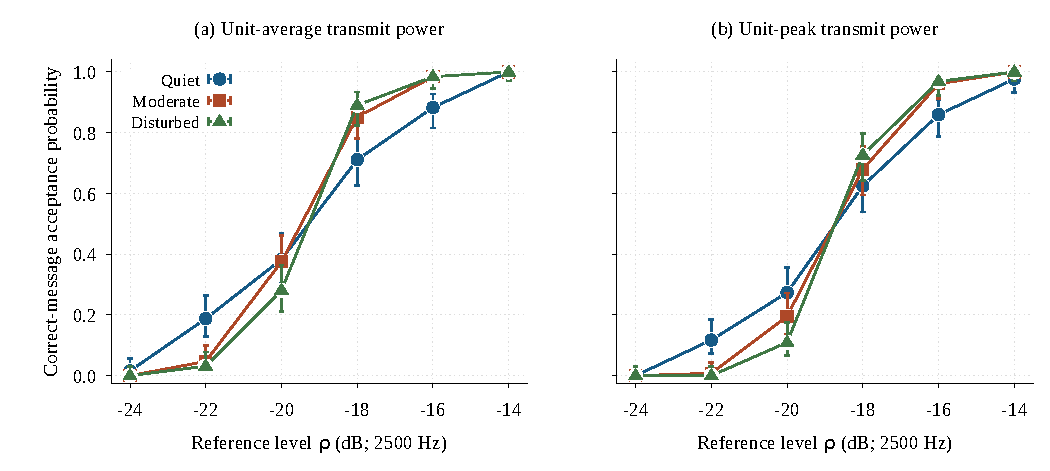
\includegraphics[width=\textwidth]{study/figures/acceptance.pdf}
\caption{Correct-message acceptance with pointwise 95\% Wilson intervals;
128 frames per point. Lines connect the measured points. The horizontal
axis is the unit-reference level $\rho$. In (a) it equals average transmit
SNR in 2500\,Hz; in (b) average transmit SNR is approximately 0.711\,dB lower.
The two panels reuse the same randomized cases.}
\label{fig:acceptance}
\end{figure}

\begin{table}[ht]
\centering\small
\begin{tabular}{@{}rll@{}}
\toprule
Reference $\rho$ & Moderate: $k/128$, rate [95\% CI] & Hard: $k/128$, rate [95\% CI] \\
\midrule
\multicolumn{3}{l}{\textit{Unit-average power}} \\
$-24$\,dB & 0/128, 0.000 [0.000, 0.029] & 0/128, 0.000 [0.000, 0.029] \\
$-22$\,dB & 2/128, 0.016 [0.004, 0.055] & 1/128, 0.008 [0.001, 0.043] \\
$-20$\,dB & 42/128, 0.328 [0.253, 0.413] & 17/128, 0.133 [0.085, 0.202] \\
$-18$\,dB & 115/128, 0.898 [0.834, 0.940] & 97/128, 0.758 [0.677, 0.824] \\
$-16$\,dB & 127/128, 0.992 [0.957, 0.999] & 127/128, 0.992 [0.957, 0.999] \\
$-14$\,dB & 128/128, 1.000 [0.971, 1.000] & 128/128, 1.000 [0.971, 1.000] \\
\midrule
\multicolumn{3}{l}{\textit{Unit-peak power}} \\
$-24$\,dB & 0/128, 0.000 [0.000, 0.029] & 0/128, 0.000 [0.000, 0.029] \\
$-22$\,dB & 0/128, 0.000 [0.000, 0.029] & 0/128, 0.000 [0.000, 0.029] \\
$-20$\,dB & 18/128, 0.141 [0.091, 0.211] & 8/128, 0.062 [0.032, 0.118] \\
$-18$\,dB & 95/128, 0.742 [0.660, 0.810] & 60/128, 0.469 [0.384, 0.555] \\
$-16$\,dB & 126/128, 0.984 [0.945, 0.996] & 123/128, 0.961 [0.912, 0.983] \\
$-14$\,dB & 128/128, 1.000 [0.971, 1.000] & 128/128, 1.000 [0.971, 1.000] \\
\bottomrule
\end{tabular}

\caption{Correct acceptances and pointwise 95\% Wilson intervals.
Every cell has zero incorrect acceptances; its erasure count is $128-k$.
Rates are dimensionless. Full erasure and incorrect-acceptance intervals
are supplied in \texttt{study/cells.csv}.}
\label{tab:cells}
\end{table}

At $-24\dB$, none of the four conditions accepts a correct message. At
$-14\dB$, every condition accepts all 128 messages; the Wilson interval
for each 128/128 cell is approximately $[0.971,1]$, so the observation does
not establish error-free operation. The transition between these limits
is resolved only at 2\,dB increments. No incorrect accepted message occurs
in any of the 3072 signal records; all remaining outcomes are erasures.
Because the power settings are paired, those records do not constitute
3072 independent opportunities for an undetected error.

\subsection{The 50\% acceptance crossing}

\begin{table}[ht]
\centering\small
\begin{tabular}{@{}llcc@{}}\toprule
Profile & Power setting & 50\% crossing & 95\% grid bracket \\
\midrule
Moderate & Average & $-19.4$\,dB & $[-20, -18]$\,dB \\
Hard & Average & $-18.8$\,dB & $[-20, -18]$\,dB \\
Moderate & Peak & $-18.8$\,dB & $[-20, -18]$\,dB \\
Hard & Peak & $-17.9$\,dB & $[-20, -16]$\,dB \\
\bottomrule\end{tabular}

\caption{Interpolated 50\% crossing in reference-level dB and conservative
95\% grid brackets under a monotone-response assumption. The bracket is
constructed from six simultaneous exact binomial intervals per curve.
Its width reflects sampling uncertainty and grid resolution.}
\label{tab:thresholds}
\end{table}

Table~\ref{tab:thresholds} places the unit-average crossings near $-19.4$
and $-18.8\dB$. Both lie between the measured $-20$ and $-18\dB$ points.
The moderate unit-peak crossing is also in that interval. For hard fading
at unit-peak power, 60/128 messages succeed at $-18\dB$, giving an
interpolated crossing near $-17.9\dB$ between $-18$ and $-16\dB$.
Its conservative uncertainty bracket spans $[-20,-16]\dB$ because the
$-18\dB$ cell does not locate the true success probability securely on
either side of 0.5. Sub-decibel interpolated values describe the chosen
interpolation and should not be read as sub-decibel measurement resolution.

\subsection{Noise-only acceptance}

\begin{table}[ht]
\centering
\begin{tabular}{@{}lrrrr@{}}
\toprule
Lot & Captures & Raw FEC accepts & Final accepts & Gate exceedances \\
\midrule
Calibration & 2048 & 0 & 0 & 21 \\
Independent check & 4096 & 0 & 0 & 44 \\
\bottomrule
\end{tabular}
\caption{Noise-only outcomes. Gate exceedance alone is not acceptance;
the receiver also requires raw decoder success.}
\label{tab:noise}
\end{table}

The independently seeded check has zero false accepts in 4096 captures,
giving the upper bound in \eqref{eq:falsebound}, or about 0.0731\% per
15-second capture. The reference scales have counts 683, 683, 683, 683,
682, and 682 in increasing $\rho$ order. The pooled bound does not supply
a separate 95\% upper limit of the same size at each scale. Both lots also
have zero raw FEC acceptances, so the evidence-only exceedances in
Table~\ref{tab:noise} must not be reported as false decoded messages.

\subsection{Waveform duration, bandwidth, and peak power}

The active waveform has exactly 116,800 samples at 12\,kHz, including both
filter tails, for a duration of 9.733333333\,s. The physical summary uses
1536 unique confirmation waveforms once each; duplicated records from the
two power settings do not enlarge the waveform sample. Mean $B_{99}$ is
1958.731\,Hz and the largest observed value is 1998.724\,Hz. Mean PAPR is
0.710905\,dB and the largest observed value is 0.710951\,dB. These extrema
belong to the sampled payloads, not to an exhaustive search of the codebook.
The nearly fixed envelope peak makes unit-peak active-frame average power
approximately 0.8490 and energy approximately 8.2636 in normalized
power-seconds, compared with 1 and 9.7333 under unit-average normalization.

\begin{figure}[ht]
\centering
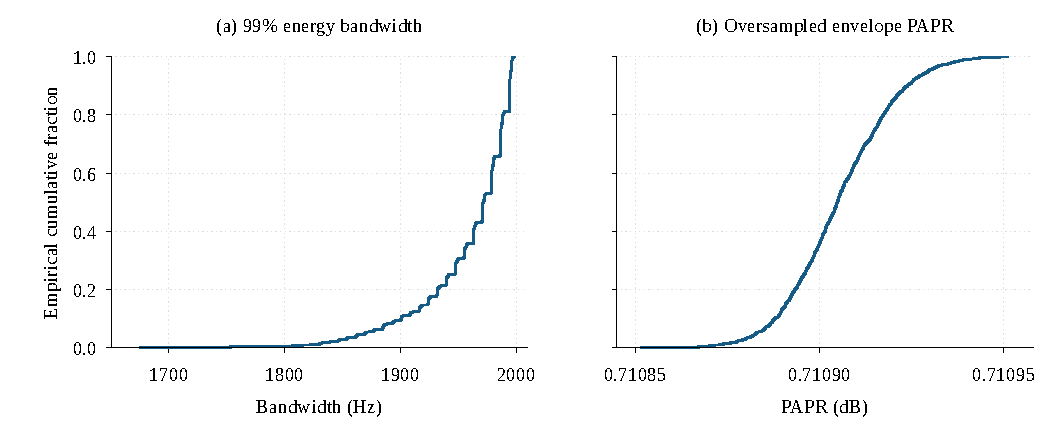
\includegraphics[width=\textwidth]{study/figures/physical.pdf}
\caption{Empirical cumulative distributions of the measured waveform
bandwidth and PAPR over 1536 unique confirmation cases. No channel fading
or noise enters these transmit-waveform measurements.}
\label{fig:physical}
\end{figure}


\section{Discussion}

The observed transition from mostly erased frames near $-22\dB$ to nearly
complete acceptance at $-16\dB$ under unit-average power is specific to the
sampled channel ensemble. The hard profile combines a larger path separation
and faster fading; the experiment changes both together and cannot isolate
their individual effects. At $-18\dB$, the correct-acceptance counts are
115/128 for moderate fading and 97/128 for hard fading. The corresponding
unit-peak counts are 95/128 and 60/128. Peak normalization reduces average
transmit power by approximately 0.711\,dB, so those two regimes must be
interpreted with their distinct reference-power conventions.

The receiver integrates each symbol without a channel estimate. Doppler
variation and delay-dependent spectral cancellation can redistribute energy
within and between its tone projections. The nonbinary decoder combines
these soft observations, but the fixed metric parameter $\gamma$ and the
fixed pilot threshold are not adapted to the individual fading realization.
The present data characterize their joint behavior; they do not identify
which stage caused each erased frame.

The guard-band estimator relies on noise in the spectral guards representing
noise in the tone region. The study uses full-band complex Gaussian noise.
Colored interference, impulsive noise, carrier drift, and other delay/Doppler
profiles were not sampled. The WAV frontend reconstructs an analytic signal
and removes part of the complex-IQ spectral support, so the reported IQ
noise statistics do not automatically describe an audio channel. These are
specific changes to the observation model that require separate measurements.

A fixed-seed estimator validation used 128 cases at every point in
Table~\ref{tab:snrvalidation}. The AWGN rows use the known transmitted payload,
so they measure the estimator without conditioning on decoder success. The
moderate and hard rows use only CRC-valid correct receiver outputs; the valid
count therefore records the available estimates. Bias is the mean of
$\widehat{\mathrm{SNR}}_{2500}$ minus the configured SNR. The AWGN absolute
bias remains below $0.08\dB$. Delay and Doppler spread energy outside the
nominal correct-tone projections, causing the increasing negative bias in the
HF profiles. The implementation applies no empirical offset to remove it.

\begin{table}[ht]
\centering
\small
\begin{tabular}{@{}lrrrr@{}}
\toprule
Channel & Target (dB) & Valid / 128 & Bias (dB) & RMSE (dB) \\
\midrule
AWGN & $-24$ & 128 & $-0.073$ & 0.892 \\
AWGN & $-22$ & 128 & $-0.080$ & 0.627 \\
AWGN & $-20$ & 128 & $-0.059$ & 0.464 \\
AWGN & $-18$ & 128 & $-0.023$ & 0.439 \\
AWGN & $-16$ & 128 & $-0.059$ & 0.286 \\
AWGN & $-14$ & 128 & $-0.026$ & 0.234 \\
Moderate & $-18$ & 115 & $-0.166$ & 0.925 \\
Moderate & $-16$ & 127 & $-0.250$ & 1.029 \\
Moderate & $-14$ & 128 & $-0.226$ & 1.002 \\
Hard & $-18$ & 104 & $-0.764$ & 1.049 \\
Hard & $-16$ & 128 & $-0.963$ & 1.318 \\
Hard & $-14$ & 128 & $-1.009$ & 1.270 \\
\bottomrule
\end{tabular}
\caption{Fixed-seed validation of the 2500\,Hz SNR estimate.}
\label{tab:snrvalidation}
\end{table}

No incorrect accepted messages occurred in the signal records, and no raw
or gated decoder acceptances occurred in the independent noise-only set.
Thus these records bound observed acceptance errors under the stated design,
but do not demonstrate an incremental reduction caused by the pilot gate.
The noise bound is pooled over six reference noise scales and is not a
uniform per-scale bound. The confirmation payload ensemble also fixes six
bits; tests of arbitrary 77-bit inputs establish functionality, while error
rates over the full payload space remain unmeasured.

\section{Implementation and reproducibility}

The standalone distribution supplies Fortran source, command-line programs,
and static and shared libraries. Headerless float32 little-endian IQ stores
interleaved I/Q samples at 12\,kHz. The optional PCM16 mono WAV frontend
uses a selectable audio center, 1500\,Hz by default. The interface guide
defines file bounds, result fields, the C layout, and serialized access to
the shared FFT cache \cite{software}. These interface details do not enter
the statistical denominators.

The study directory contains the per-trial signal and noise records, their
checksums and provenance, the channel implementation and single-trial
reproduction harness, and a Fortran analysis program. Its commands regenerate
the cell tables and plotting data; the plotting script renders those results
without recomputing the statistics \cite{study}.

A clean GNU Fortran/C build and the regression suite verify the
implementation separately from the performance study. The suite
passes 88 core checks, 26 I/O checks, and 39 CLI checks, together with Fortran
and C API roundtrips. These are assertion counts, not channel trials. The
fixed-seed SNR validation is a separate executable and reports all cases in
Table~\ref{tab:snrvalidation}. The regression suite also
matches the retained codeword, complete CF32 frame, and PCM waveform fixtures.
The exact CF32 roundtrip checks the integer representations of quantized
samples. Strict compilation treats compiler warnings as errors
\cite{verification}.

The code is distributed under GPL-3.0-or-later. Nico Palermo's graph,
coefficient, algorithm and metric attribution and the relevant source-package
identifiers are retained in \path{licenses/QRA-NOTICE.txt}. Checksums identify
the delivered source and data.

\section{Conclusion}

QF256 transmits a 77-bit message in a 9.733333-second filtered 256-tone burst
and combines blind pilot acquisition with nonbinary soft decoding and a
fixed acceptance rule. CRC-valid outputs include a 2500\,Hz-referenced SNR
estimate whose AWGN behavior and dispersive-channel bias are quantified above.
The completed HF study provides cell-level success
estimates and uncertainty under two specified fading profiles and two power
constraints. The independent noise check provides a finite-sample bound on
false acceptance, while waveform measurements quantify bandwidth and peak
power. The accompanying records and analysis code reproduce the reported
tables and figures.

\appendix
\section{Graph specification}
\label{app:graph}

The input indices $v_i$, $i=1,\ldots,51$, for
\eqref{eq:accumulator}--\eqref{eq:termination} are the following sequence,
read left to right and top to bottom:
\begin{center}\small\ttfamily
\begin{tabular}{@{}l@{}}
14, 2, 4, 5, 9, 13, 10, 15, 11, 6, 1, 8, 2, 12, 9, 10, 13,\\
7, 4, 11, 8, 6, 3, 14, 13, 5, 9, 1, 2, 12, 3, 10, 15, 6,\\
7, 14, 8, 13, 12, 3, 10, 1, 11, 5, 8, 15, 9, 12, 4, 7, 11
\end{tabular}
\end{center}
The coefficient exponents $\ell_i$ are:
\begin{center}\small\ttfamily
\begin{tabular}{@{}l@{}}
0, 14, 0, 0, 13, 37, 0, 27, 56, 62, 29, 0, 52, 34, 62, 4, 3,\\
22, 25, 0, 22, 0, 20, 10, 0, 43, 53, 60, 0, 0, 0, 62, 0, 5,\\
0, 61, 36, 31, 61, 59, 10, 0, 29, 39, 25, 18, 0, 14, 11, 50, 17
\end{tabular}
\end{center}
To construct $h_i$, first generate the powers of element 2 in
$\GF(64)$ using polynomial \texttt{0x43}, and take the integer value
represented by the six-bit element at exponent $\ell_i$. Embed that
integer as the corresponding eight-bit polynomial element of $\GF(256)$.
The numbers $\ell_i$ are therefore \emph{not} used directly as logarithms
in $\GF(256)$. The literal arrays and this conversion are preserved in
the shipped coding source \cite{coding}.

\begin{thebibliography}{99}
\bibitem{sumproduct}
F. R. Kschischang, B. J. Frey, and H.-A. Loeliger,
``Factor graphs and the sum-product algorithm,''
\emph{IEEE Transactions on Information Theory}, vol. 47, no. 2,
pp. 498--519, 2001. \href{https://doi.org/10.1109/18.910572}{doi:10.1109/18.910572}.

\bibitem{watterson}
C. C. Watterson, J. R. Juroshek, and W. D. Bensema,
``Experimental confirmation of an HF channel model,''
\emph{IEEE Transactions on Communication Technology}, vol. 18, no. 6,
pp. 792--803, 1970.
\href{https://doi.org/10.1109/TCOM.1970.1090438}{doi:10.1109/TCOM.1970.1090438}.

\bibitem{wilson}
E. B. Wilson, ``Probable inference, the law of succession, and statistical
inference,'' \emph{Journal of the American Statistical Association},
vol. 22, no. 158, pp. 209--212, 1927.
\href{https://doi.org/10.1080/01621459.1927.10502953}{doi:10.1080/01621459.1927.10502953}.

\bibitem{clopper}
C. J. Clopper and E. S. Pearson, ``The use of confidence or fiducial limits
illustrated in the case of the binomial,'' \emph{Biometrika}, vol. 26,
no. 4, pp. 404--413, 1934.
\href{https://doi.org/10.1093/biomet/26.4.404}{doi:10.1093/biomet/26.4.404}.

\bibitem{physical}
QF256, \emph{Physical modem implementation}, version 1.0.0,
\path{src/core/mfsk_iq.f90} and \path{src/core/waveform_metrics.f90}.

\bibitem{coding}
QF256, \emph{Nonbinary coding implementation}, version 1.0.0,
\path{src/core/qra_soft.f90}.

\bibitem{software}
QF256, \emph{Standalone implementation and interface documentation},
version 1.0.0, \path{README.md}, \path{docs/API.md},
\path{src/qf256_api.f90}, and \path{include/qf256.h}.

\bibitem{study}
QF256, \emph{HF confirmation and noise-only study records and analysis},
October 2026, \path{study/}. Data, source and reproduction instructions
in the accompanying distribution.

\bibitem{verification}
QF256, \emph{Build, regression and source-integrity records}, October 2026,
\path{docs/VALIDATION.txt}, \path{docs/CORE.sha256}, and
\path{docs/DELIVERY.sha256}.

\bibitem{provenance}
N. Palermo, \path{qra15_65_64_irr_e23.c} (2020) and
\path{qracodes.c} (2016), QRA graph and decoder sources,
GPL-3.0-or-later. Source package: WSJT-X 2.7.0+repack-1,
\href{https://sources.debian.org/src/wsjtx/2.7.0\%2Brepack-1/lib/qra/q65/}{Debian Sources, lib/qra/q65},
retrieved October 10, 2026. Attribution and encoding references are preserved
in \path{licenses/QRA-NOTICE.txt}.

\end{thebibliography}
\end{document}
